We continue with our quest of generalizing multivariable calculus.
The next familiar object waiting to be questioned are vector fields.
In the euclidean settings these are simply continuous maps that attach a vector to each point in their domain.

The step to abstract manifold is rather intuitive in this case: a vector field will be a map that, at each point of a manifold, picks a tangent vector at that point in a smooth way.

\begin{definition}\label{def:vfield}
  A $C^p$-map $X: M \to TM$ with $\pi\circ X = \id_M$, or equivalently $X_p\in T_pM$ for all $p\in M$, is called \emph{$C^p$-vector field}.
  We denote\footnote{Alternative notations are $\cT_0^1(M)$, $\cT(M)$ and $\Gamma(TM)$. The first two are related to vector fields being tensor fields of type $(1,0)$, a topic that we will discuss in the near future.} the set of smooth vector fields by $\fX(M)$.

  The map $\pi:TM \to M$ is called \emph{footpoint map} and, for reasons that will be clear later on, the equation $\pi\circ X = \id_M$ is called \emph{section property}.
\end{definition}

\begin{remark}
  A careful look at the definition shows that vector fields are sections of $TM$, indeed $\fX(M) \equiv \Gamma(TM)$.
  This is a useful way to start understanding the bundle terminology: in some sense, sections of vector bundles are a generalisation of vector fields.
\end{remark}

Beware of the curse of differential geometry.
For convenience and to be consistent with our notation for elements of the tangent bundle, we denote the value $X_p\in\{p\}\times T_p M$ of a vector field by $X_p$ instead of $X(p)$.
Furthermore, we will often identify $X_p$ with its component in $T_pM$, thus considering it as if $X_p\in T_pM$, without explicitly projecting it to the second component.

Let $M$ be a smooth $n$-manifold (with or without boundary).
Let $X:M\to TM$ be a vector field, not necessarily smooth, and $(U, (x^i))$ a smooth coordinate chart for $M$. Then we can write the value of $X$ at any point $p\in U$ as a linear combination in terms of the coordinate basis vector:
\begin{equation}\label{eq:vfCoordBAsis}
  X_p = X^i(p) \frac{\partial}{\partial x^i}\Big|_p.
\end{equation}
This defines $n$ functions $X^i: U\to\R$, called \emph{component functions of $X$} in the chart.

\begin{exercise}
  Show that, in the notation above, the restriction of $X$ to $U$ is smooth if and only if its component functions with respect to the chart are smooth.
\end{exercise}

\begin{example}
  If $(U, (x^i))$ is a smooth coordinate chart for a manifold $M$, the assignment $p \mapsto \frac{\partial}{\partial x^i}\big|_p$ determines a vector field on $U$, called the \emph{$i$th-coordinate vector field} and commonly denoted $\partial_{i}$, $\partial_{x^i}$ or $\partial/\partial x^i$.
  Despite their looks, the $\partial_{x^i}|_p$ denote genuine vectors in $T_p M$ that can be associated to euclidean vectors via a suitable chart.
\end{example}

The space of smooth vector fields is a vector space under pointwise addition and scalar multiplication: for all $p\in M$, $X,Y\in\fX(M)$, $\alpha, \beta \in \R$, we have
\begin{equation}
  (\alpha X + \beta Y)_p = \alpha X_p + \beta Y_p.
\end{equation}
The zero element of the vector space, called \emph{zero vector field}, is the vector field whose values is $0\in T_pM$ for all $p\in M$.
Moreover, each vector field can be multiplied by smooth functions $f\in C^\infty(M)$ by defining $fX:M\to  TM$ by
\begin{equation}
  (fX)_p = f(p)X_p.
\end{equation}

\begin{proposition}
  Let $M$ be a smooth manifold with or without boundary.
  \begin{enumerate}
    \item If $X,Y \in \fX(M)$ and $f,g\in C^\infty(M)$, then $fX+gY \in\fX(M)$.
    \item $\fX(M)$ is a module over the ring $C^\infty(M)$.
  \end{enumerate}
\end{proposition}

In this sense, the basis expression \eqref{eq:vfCoordBAsis} can be also rewritten as an equation between fields instead of an equation between vectors at point:
\begin{equation}\label{eq:vfCoordBAsis}
  X = X^i \frac{\partial}{\partial x^i},
\end{equation}
where $X^i$ denotes the component of the vector field $X$ in the given coordinates.

There is one more way of thinking about the coordinate basis expression above.
We have seen that differentials of smooth maps define maps between tangent bundles.
As it turns out, we can employ differentials of diffeomorphisms to map vector fields to vector fields.

\begin{definition}
  Let $F:M\to N$ be a diffeomorphism of smooth manifolds.
  Then, the \emph{pushforward} $F_*$ of $F$, defined by\footnote{In coordinates, this reads\begin{equation}
      (F_* X)_q = dF_{F^{-1}(q)}(X_{F^{-1}(q)}).
    \end{equation}}
  \begin{equation}
    F_*: \fX(M) \to \fX(N),\qquad
    X \mapsto F_* X = d F \circ X \circ F^{-1},
  \end{equation}
  maps (``pushes forward'') vector fields on $M$ to vector fields on $N$.
\end{definition}

The definition of pushforward is more easily pictured by means of the following commutative diagram:
\begin{equation}
  \begin{tikzcd}[row sep=huge, column sep=huge]
    M \arrow[d, "X"]
    & N \arrow[l, "F^{-1}"] \arrow[d, "F_*X" cyan]\\
    TM \arrow[r, "d F"]
    & TN
  \end{tikzcd}.
\end{equation}

Then, if $(U, \phi)$ is a coordinate chart for $M$, the restriction of a vector field $X\in\fX(M)$ to $U$ can be mapped to a vector field on $\phi(U)\subset\R^n$ via the pushforward $\phi_*$:
\begin{align}
  \phi_* X & : \LaTeXunderbrace{\phi(U)}_{\subset\R^n} \to \LaTeXunderbrace{T \phi(U)}_{=\phi(U)\times\R^n}, \\
  \phi_* X & : x\mapsto (q,v(x)) \quad\mbox{with}\quad v(x) = v^j(x)e_j \in \R^n,
\end{align}
where $v^j(x)$ are the components\footnote{As we start getting used to, the chart $\phi$ here plays a twofold role: it provides the coordinates $x=\phi(p)$ on the patch $U$ and the coordinate basis of the tangent space.} of $X_p\in T_p M$ at $p=\phi^{-1}(x)$ with respect to the coordinate basis $\left\{\frac{\partial}{\partial x^i}\big|_x\right\}$.

\todo{Example 8.20 Lee + Corollary 8.21}

% XXX: Remember to mention it when we define pullbacks
% An interesting property of the pushforward defined above is that
% \begin{equation}
%     X(f\circ F) = F_*X(f) \circ F, \quad f\in C^\infty(N).
% \end{equation}

% Indeed,
% \begin{align}
%     X(f^* F) = d (f\circ F) \circ X = df \circ dF \circ X = df \circ F_* X \circ F = F_* X (f) \circ X.
% \end{align}
% This is called natural behavior: either you can pull back the function $f$ to $M$ or push forward the vector field $X$ to $N$.

While we continue to explore the twofold nature of geometric objects, it is worth looking back at our original definition of tangent vectors.
In one of our first encounters with tangent spaces, we said that a tangent vector $v$ at a point $p\in M$ defines a derivative at that point by taking the directional derivative of a function at that point.
\marginnote{Clearly all of the definitions above hold if instead of $M$ we consider open subsets $U\subset M$.}
A vector field $X$ now provides a tangent vector and, therefore, a derivation at every point of the manifold.
In this sense, $X\in\fX(M)$ induces a linear map on the algebra $C^\infty(M)$ of smooth functions on $M$: for $f\in C^\infty(M)$,
\begin{equation}\label{eq:diff_directional_derivative}
  Xf : M\to\R, \quad
  (Xf)_p := X_p f, \quad p\in M.
\end{equation}
\marginnote{Beware of the ordering: $fX\in\fX(M)$ but $Xf\in C^\infty(M)$!}

\begin{notation}\label{notation:derivative}
  Let $f\in C^\infty(M)$ and let $(U, \phi)$ be a chart with coordinates $(x^i)$.
  Then, for $X = \frac{\partial}{\partial x^i}$, we denote $Xf$ by $\frac{\partial f}{\partial x^i}$ and thus the following notations are for us equivalent:
  \begin{equation}
    \frac{\partial f}{\partial x^i}(p)
    = \left(\frac{\partial}{\partial x^i}\right)_p(f)
    = \frac{\partial}{\partial x^i}\Big|_p(f)
    = D_i(f\circ\phi^{-1})(\phi(p)).
  \end{equation}
  If $M$ is an open subset of $\R^n$ and $\phi=\id_{\R^n}$, then the last equality shows that the notation is consistent with the usual definition of partial derivatives from multivariable analysis.
\end{notation}

\begin{exercise}
  If $X\in\fX(M)$ and $f\in C^\infty(M)$, then $Xf\in C^\infty(M)$.
\end{exercise}

This whole discussion allows us to extend the notion of derivation at a point to a derivation on the whole space.
\begin{definition}
  Let $M$ be a smooth manifold and $\emptyset\neq W\subset M$ an open set.
  A \emph{derivation on $C^\infty(W)$} is a linear map
  \begin{equation}
    \cX:C^\infty(W)\to C^\infty(W)
  \end{equation}
  satisfying Leibniz rule:
  \begin{equation}
    \cX(fg) = f \cX(g) + g \cX(f).
  \end{equation}
\end{definition}

Any vector field $X\in\fX(W)$ defines a derivation $\cX$ via $\cX(f) = Xf$. In fact the opposite is also true:
\begin{proposition}
  Let $M$ be a smooth manifold and $\emptyset\neq W\subset M$ an open set.
  The set of derivation on $W$ and $\fX(W)$ are isomorphic as $C^\infty(W)$-modules.
\end{proposition}
\begin{proof}
  Suppose $\cX$ is a derivation on $C^\infty(W)$ and fix $p\in W$. Then $\cX$ defines a derivation on $C^\infty(W)$ at $p$, which we casually denote by $X_p$, via the formula
  \begin{equation}
    X_p(f) := \cX(f)(p), \quad\forall f\in C^\infty(W).
  \end{equation}
  We can then think of $X$ as a map $W\to TM$ via $X\mapsto X_p$.
  \marginnote{Challenge: count how many times we are using the isomorphism between derivations at points and tangent vectors in this proof.}
  Since $X(f)=\cX(f)$ by construction, it is a smooth function for all $f\in C^\infty(W)$ and therefore is smooth as vector field, concluding the proof.
\end{proof}

Therefore, from now on, we will also interchange derivations of $C^\infty$ and vector fields, and call them with capital latin letters.

\section{Lie brackets}

Once you have a module, it is worth checking if you can get an algebra.
Indeed, that is going to be our next objective.
To this end, we look for a bilinear map $\fX(W)\times\fX(W) \to \fX(W)$.

The most natural choice is to just compose the vector fields, that is, apply the derivatives one after the other:
\begin{equation}
  X Y := X \circ Y : C^\infty(W) \to C^\infty(W), \quad
  (X Y)(f) := X(Y(f)).
\end{equation}
If this satisfies the product rule, we are done.
Let $f,g\in C^\infty(W)$, we have
\begin{align}
  (X Y)(fg) &= X(fY(g) + gY(f)) \\
  &= \left(f(X Y)(g) + g(X Y)(f)\right) + \left( X(f)Y(g) +X(g)Y(f)\right).
\end{align}
Unfortunately for us, this is not a derivation. However, we do not seem to be so far off.
If we carefully look at the ``error'', i.e. the term $\left( X(f)Y(g) +X(g)Y(f)\right)$, we can observe that it is symmetric with respect to $X$ and $Y$.
One way to let it cancel out, is to consider the \emph{commutator} of the two vector fields:
\begin{equation}\label{def:commutator}
    [X,Y] := X Y - Y X.
\end{equation}
Indeed, $[X,Y]$ is a derivation.

\marginnote{Do not confound Lie with lie. Here Lie is the surname of Sophus Lie, an important Norwegian mathematician that lived in the second half of the 19th century.}
\begin{definition}
    Let $X,Y\in\fX(W)$. We call \emph{Lie bracket} of $X$ and $Y$ the derivation given by their commutator $[X,Y] := X Y - Y X$.
\end{definition}

\begin{remark}
  Note that the Lie brackets are \emph{not} uniquely determined by $X_p$ and $Y_p$: the smooth functions $X(f)$ and $Y(f)$ depend on the values of $X$ and $Y$ in a neighbourhood of $p$.
\end{remark}

\begin{exercise}\label{ex:vfliealgebra}
  Show that the Lie bracket $[,]$ of vector fields satisfies the following properties. Let $X,Y,Z\in\fX(M)$:
  \begin{enumerate}[(i)]
    \item (antisymmetry) $[X, Y] = - [Y, X]$;
    \item (bilinearity) $[\alpha X + \beta Y, Z] = \alpha [X, Z] + \beta [Y, Z]$ and $[X, \alpha Y + \beta Z] = \alpha [X, Y] + \beta [X, Z]$, for all $\alpha,\beta \in\R$;
    \item (\emph{Jacobi identity}) $[X,[Y,Z]] + [Y,[Z,X]] + [Z,[X,Y]] = 0$.
  \end{enumerate}
\end{exercise}

\begin{proposition}
  For all $X, Y \in \fX(M)$ and for all $f,g\in C^\infty(M)$,
  \begin{equation}
    [fX, gY] = fg[x,y] + f(Xg)Y - g(Yf)X.
  \end{equation}
\end{proposition}
\begin{exercise}
  Prove the proposition.
\end{exercise}

We will see many applications of the Lie brackets throughout the rest of the course, but before doing anything, let's find an effective way to compute it.

\begin{proposition}
    Let $(U, \phi)$ be a chart on $M$ with local coordinates $(x^i)$ and let $X,Y\in\fX(U)$.
    If $X = X^i \frac{\partial }{\partial x^i}$ and $Y = Y^i \frac{\partial}{\partial x^i}$ are the coordinate expressions for $X$ and $Y$, then\footnote{Recall Notation~\ref{notation:derivative}!}
    \begin{equation}
        [X,Y] = \left(X^i\frac{\partial Y^j}{\partial x^i} - Y^i\frac{\partial X^j}{y^i}\right)\frac{\partial}{\partial x^j}.
    \end{equation}
\end{proposition}
\begin{exercise}
  Prove the proposition.
\end{exercise}

\begin{theorem}\label{thm:liealgiso}
  Let $F:M\to N$ be a diffeomorphism between smooth manifolds with or without boundary and let $X, Y \in\fX(M)$. Then,
  \begin{equation}
    \left((F_* X)f\right)\circ F = X(f\circ F), \quad\mbox{and}\quad
    F_* [X,Y] = [F_* X, F_* Y].
  \end{equation}.
\end{theorem}
\begin{proof}
  By definition, for $f\in C^\infty(N)$, $X\in\fX(M)$ and any $p\in M$
  \begin{align}
    X(f\circ F)(p) &= X_p(f\circ F) \\
    &= dF_p(X_p)f = (F_* X)_{F(p)}f \\
    &= (F_*X f)(F(p)) = (F_*X f)\circ F(p).
  \end{align}
  Which proves the first equation.
  Therefore,
  \begin{align}
    X Y (f\circ F) = X ((F_* Y) f \circ F) 
    = ((F_* X) (F_* Y) f) \circ F,
  \end{align}
  and similarly for $Y X$.
  Finally, by definition we have
  \begin{align}
    (F_* [X,Y] f)\circ F
    &= [X,Y](f\circ F) \\
    &= XY (f\circ F) - YX (f\circ F) \\
    &= ((F_* X) (F_* Y)f)\circ F - ((F_* Y) (F_* X)f)\circ F\\
    &= ([F_* X, F_* Y]f)\circ F,
  \end{align}
  completing the proof.
\end{proof}

\begin{definition}\label{def:LieAlgebra}
  A \emph{Lie algebra} (over $\R$) is a real vector space $\fg$, endowed with a bilinear antisymmetric map
  \begin{equation}
    \fg \times \fg \to \fg, \quad (v,w)\mapsto [v,w],
  \end{equation}
  called \emph{Lie bracket}, which in addition satisfies the Jacobi identity\footnote{Thus a Lie algebra is a non-associative algebra.}. 
  The \emph{dimension} of the Lie algebra is the dimension of $\fg$ as a vector space.

  If $\fg$ is a Lie algebra, then a linear subspace $\fh\subset\fg$ is called a \emph{Lie subalgebra} if $[v,w]\in\fh$ for all $v,w\in\fh$.
\end{definition}

\begin{example}
  Exercise~\ref{ex:vfliealgebra} shows that the space $\fX(M)$ of vector fields on a manifold $M$ is a Lie algebra.
  Since $\fX(M)$ is a $C^\infty(M)$-module and $C^\infty(M)$ is an infinite-dimensional vector space, it defines an infinite dimensional Lie algebra.

  This may seem an alien concept at first, however there are many simple examples of Lie algebras. To name a few:
  \begin{enumerate}
    \item $\R^3$ with the cross product $[x,y]:=x\times y$ is a $3$-dimensional Lie algebra;
    \item the set $\mathrm{Mat}(n)$ of $n\times n$-matrices with the matrix commutator $[A,B] = AB-BA$ is a $n^2$-dimensional Lie algebra, usually denoted $\mathfrak{gl}(n\R)$;
    \item any vector space $V$ turns into an (abelian) Lie algebra by defining $[v,w]=0$;
    \item if $V$ is a vector space, the vector space of all linear maps from $V$ to itself becomes a Lie algebra, denoted $\mathfrak{gl}(V)$, with the brackets defined by $[A,B] = A\circ B-B\circ A$. Note that with the usual identification of $n\times n$ matrices with linear maps from $\R^n$ to itself, $\mathfrak{gl}(\R^n)$ coincides with $\mathfrak{gl}(n, \R)$.
  \end{enumerate}
\end{example}

\begin{definition}
  Let $\fg$ and $\fh$ be two Lie algebras. A \emph{Lie algebra homomorphism} is a linear map $T:\fg\to\fh$ which preserves the Lie brackets, i.e.
  \begin{equation}
    [Tv, Tw]_\fh = T[v,w]_\fg, \quad \forall v,w\in\fg.
  \end{equation}

  A \emph{Lie algebra isomorphism} is a bijective Lie algebra homomorphism whose inverse is also a Lie algebra homomorphism.
\end{definition}

In Theorem~\ref{thm:liealgiso} we have thus shown that the pushforward is a Lie algebra isomorphism!

\section{Flows and integral curves}

Once again, a comparison with the euclidean world can open the door to a whole new world.
Vector fields on euclidean spaces give rise to ordinary differential equations (ODEs) and to each vector field we can associate a flow, that is, the curve that solve the ODE.

The classical theorems of existence and uniqueness of solutions of ODEs, then, give us the necessary conditions to ensure that such flow exists locally or globally and it is well defined.
For a rather detailed account you can refer to \cite[Chapters 3.2 and 3.3]{book:knauf} (which you can freely access on \href{https://link.springer.com/book/10.1007\%2F978-3-662-55774-7}{SpringerLink} via the university proxy).

In fact, if $X: U\subset\R^n \to \R^n$ is a vector field on an open subset $U$ of $\R^n$, and
\begin{equation}\label{eq:XflowRn}
  \dot u(t) = X(u(t))
\end{equation}
is the corresponding ODE, then we have the following implications of the euclidean theorems on existence and uniqueness of solutions:
\begin{enumerate}[(i)]
  \item if $X$ is continuous, then for each $x\in U$ there exists $\epsilon > 0$ and a differentiable curve $u = u_{x} : (-\epsilon, \epsilon) \to U$ with $u_x(0) = x$ that solves \eqref{eq:XflowRn};
  \item (Picard-Lindel\"of theorem) if $X$ is locally Lipschitz continuous, then the solution $u_x$ is unique;
  \item if $X\in C^p(U,\R^n)$, then the solution map $\Phi : (t, x) \to (t, x) := u_x (t)$ is $p$-times continuously differentiable as a function of the initial data, i.e. $\Phi(x, \cdot)\in C^p(U)$ for all $t$ in the existence domain.
\end{enumerate}

As we are getting used to, the whole theory can be extended to manifolds in a quite direct but perhaps surprising fashion.

\begin{definition}
  Let $M$ be a manifold and let $X\in\fX(M)$.
  A smooth curve $\gamma: (a,b)\subset\R \to M$ is an \emph{integral curve} of $X$ if
  \begin{equation}\label{eq:integralCurve}
    \gamma'(t) = X_{\gamma(t)} \qquad \forall t\in(a,b).
  \end{equation}
  Conventionally, we assume that $0\in(a,b)$. In this case, if $\gamma(0)=p$, we say that $\gamma$ is an integral curve \emph{through $p$}.
\end{definition}

\begin{example}
  \todo{Lee Example 9.1 p. 206}
\end{example}

\begin{notation}
  If $M$ is a manifold and $(a,b)\subset\R$, also $(a,b)\times M$ is a manifold. 
  Conventionally, for $p\in M$ we will denote $i_p : (a,b) \to (a,b)\times M$ the map $i_p(t) := (t,p)$.
  All the following notations will denote the tangent vector in $T_{(t,p)}((a,b)\times M)$ obtained from $\frac{\partial}{\partial t}\big|_t \in T_t\R$:
  \begin{equation}
    \frac{\partial}{\partial t}\Big|_{(t,p)} := d (i_p)_t\left(\frac{\partial}{\partial t}\Big|_t\right) = \frac{d}{d t}  i_p(t) = i_p'(t).
  \end{equation}
\end{notation}

Exercise~\ref{ex:tg_curve_iso} implies that in the euclidean case our definition (in terms of equality of tangent vectors on $T_{\gamma(t)}(M)$) coincides with the euclidean flow (defined in terms of equality of real numbers).
Alternatively, one can pick a coordinate chart and use the pushforward to locally compare the definitions.

Indeed, if $(U, \phi)$ is a chart with coordinates\footnote{We will soon stop being so verbose and just write ``in local coordinates on $U$'' without specifying their names (unless strictly necessary)!} $(x^i)$, let $\gamma(t) = (\gamma^1(t), \ldots, \gamma^n(t))$ in these coordinates. Then, condition \eqref{eq:integralCurve} above can be written as
\begin{equation}
  \dot\gamma^i(t)\frac{\partial}{\partial x^i}\Big|_{\gamma(t)}
  = X^i(\gamma(t))\frac{\partial}{\partial x^i}\Big|_{\gamma(t)},\quad i=1,\ldots,n,
\end{equation}
where we use the dot to denote the derivative in $t$ for readability.
These equations can be further rewritten as the system of partial differential equations of the same form as \eqref{eq:XflowRn}
\begin{equation}
  \begin{cases}
    \dot\gamma^1(t) = X^1(\gamma^1(t), \ldots, \gamma^n(t)) \\
    \quad \vdots \\
    \dot\gamma^n(t) = X^n(\gamma^1(t), \ldots, \gamma^n(t))
  \end{cases},
\end{equation}
to which we can apply euclidean theorems of existence and uniqueness!
Note also the terminology here, an ``integral curve'' for $X$ is the curve you obtain ``integrating'' the system of ODE associated to $X$.

This immediately implies the following theorem.

\begin{theorem}[Existence, uniqueness and differentiability of local solutions] %
  \label{thm:exuniqloc}
  Let $M$ be a smooth manifold and $X\in\fX(M)$. For every $x\in \circ M := M\setminus \partial M$, there exists $\epsilon > 0$, an open neighbourhood $U\subset\circ M$ of $x$ and a unique map $\Phi : (-\epsilon, \epsilon) \times U \to M$, $(t, p) \mapsto \Phi(t,p)$, such that
  \begin{enumerate}[(i)]
    \item for every $p\in U$, the curve $\Phi_p : (-\epsilon, \epsilon) \to M$, $t\mapsto \Phi_p(t) := \Phi(t, p)$ is an integral curve of $X$ through $p$, that is, $\Phi_p' = X\circ\Phi_p$ and $\Phi_p(0) = p$;
    \item for every $t\in(-\epsilon, \epsilon)$, the map $\Phi_t: U \to M$, $p\mapsto \Phi_t(p):=\Phi(t,p)$, is a diffeomorphism from $U$ onto an open subset of $M$.
  \end{enumerate}
\end{theorem}
  
\begin{remark}
  In some text, instead of $\Phi_p' = X\circ\Phi_p$, you read
  \begin{equation}
    d\Phi_{(t,p)}\left(\frac{\partial}{\partial t}\Big|_{(t,p)}\right) = X \circ \Phi(t,p).
  \end{equation}
  This should not scare you since by definition
  \begin{equation}
    d\Phi_{(t,p)}\left(\frac{\partial}{\partial t}\Big|_{(t,p)}\right) = (\Phi \circ i_p)'(t) = \Phi_p'(t).
  \end{equation}
\end{remark}

We call the map $\Phi$ a \emph{local flow} of $X$.
If a local flow is defined on $\R\times M$, we call it a \emph{global flow} and the associated vector field is called a \emph{complete vector field}.

\begin{example}\label{example:lineardrift}
  Let $M=\R^n$ and $L\in\fX(M)$ defined by $L(p^1, \ldots, p^n) = (p^1, \ldots, p^n, 1, 0, 0, \ldots, 0)$.
  Then $\Phi^L$ is a global flow, explicitly given as
  \begin{equation}
    \Phi^L(t,p) = (p^1+t, p^2, \ldots, p^n).
  \end{equation}
  Such flow $\Phi^L$ is called \emph{linear drift}.
\end{example}

Every smooth vector field has a local flow about any point, but not necessarily a global flow.
\begin{example}[A global flow may not exist]\label{ex:non-complete}
  Let $M = R^2$ and $X = x^2 \frac{\partial}{\partial x}$.
  Then, the unique integral curve of $X$ starting a $(1,0)$ is
  \begin{equation}
    \gamma(t) = \left(\frac{1}{1-t}, 0\right).
  \end{equation}
  Since $i_x \circ \gamma(t)$ is unbounded as $t\to 1$, this curve cannot be extended past $t=1$.

  A somewhat simpler example is given by the vertical lines on $\cH^2$ (so a manifold with boundary). These are integral curves of $\frac{\partial}{\partial x^2}$ which cannot extend further than the boundary $\{x^2=0\}$.
\end{example}

The previous theorem, in particular, implies that if $\gamma, \delta : (a,b)\to M$ are integral curves of $X$ with $\gamma(t) = \delta(t)$ for some $t \in(a,b)$, then $\gamma\equiv\delta$.

This justifies the following definition.
\begin{definition}
  Let $M$ be a smooth manifold and $X\in\fX(M)$.
  For a given $p\in M$, we denote $I_p = \left(t^-(p), t^+(p)\right) \subset\R$, $0 \in I_p$, the maximal interval on which the unique integral curve $\gamma_p : I_p \to M$ of $X$ through $p$ is defined.
  We call such curve $\gamma_p$ the \emph{maximal integral curve through $p$}.
\end{definition}

\begin{remark}
  It follows from the definition of maximality that for any $p\in M$ one has
  \begin{equation}
    t^{\pm}(\gamma_p(s)) = t^\pm(p) - s \qquad \forall s\in I_p.
  \end{equation}
\end{remark}

Note that $I_p$ is typically larger than the domain of definition $(-\epsilon, \epsilon)$ of $\Phi_p$. By construction $\Phi_p$ never leaves the coordinate set $U$ over which it was defined, on the other hand $\gamma_p$ can in general wander all over the manifold -- even though $\gamma_p = \Phi_p$ for small enough $t$!

Again, theorems about existence and uniqueness of euclidean maximal flows imply that we can extend $\Phi_p$ uniquely to a maximal flow.

\begin{theorem}[Existence and uniqueness of maximal solutions] %
  \label{thm:exuniqmax}
  Let $M$ be a smooth manifold and $X\in\fX(M)$.
  There exists a unique open set $\cD \subset \R\times\circ M$ and a unique smooth map $\Phi:\cD\to M$ such that
  \begin{enumerate}[(i)]
    \item\label{thm:exuniqmax:i} for all $p\in M$ one has $\cD\cap(\R\times\{p\}) = I_p\times\{p\}$;
    \item\label{thm:exuniqmax:ii} $\Phi(t,p) = \gamma_p(t)$ for all $(t,p)\in\cD$.
  \end{enumerate}
\end{theorem}

We call $\Phi$ the \emph{flow} of $X$.
When we want to emphasize the vector field $X$, we will write $\Phi^X$.

\begin{proof}
  Both $\cD$ and $\Phi$ are uniquely identified respectively by (\ref{thm:exuniqmax:i}) and (\ref{thm:exuniqmax:ii}), so to prove the thoerem one only needs to show that $\cD$ is open and that $\Phi$ is smooth.
  This is done by applying the euclidean theorems to extend the local flow, finally showing that for all $p\in M$ and $t\in I_p$, $\cD$ contains a neighbourhood of $(t,p)$ on which $\Phi$ is smooth.

  We are going to omit the details of the proof, the interested reader can refer to \cite[Proposition 9.12]{book:lee}.
  The statement may seem different at a first glance, but a careful look will reveal that he is just taking a slightly different perspective.

  Indeed, if we reverse the roles of $t$ and $x$, we can define for any given $t\in M$ the set
  \begin{equation}
    M_t := \{p\in M \;\mid\; (t,p)\in\cD\}.
  \end{equation}
  Then Theorem~\ref{thm:exuniqmax} is equivalent to say that $M_t$ is open in $M$, $M = \cup{t>0} M_t$, and there is a well-defined smooth map $\Phi_t : M_t \to M_{-t}$ given by
  \begin{equation}\label{eq:flowdiffeo}
    \Phi_t(p) := \Phi(t,p), \quad p\in M_t.
  \end{equation}
  Which is exactly the claim in \cite[Proposition 9.12]{book:lee}.

%   Both $\cD$ and $\Phi$ are uniquely identified respectively by (\ref{thm:exuniqmax:i}) and (\ref{thm:exuniqmax:ii}), so we only need to show that $\cD$ is open and that $\Phi$ is smooth.
%   To this end we are going to prove that for all $p\in M$ and $t\in I_p$, $\cD$ contains a neighbourhood of $(t,p)$ on which $\Phi$ is smooth.

%   Fix $p\in M$ and denote $J\subset I_p$ the set of all $t\in I_p$ for which there is some neighbourhood of $(t,p)$ contained in $\cD$ on which $\Phi$ is smooth. Since this is an open condition, the set $J$ is open and by Theorem~\ref{thm:exuniqloc}, $0\in J$, so $J$ is not empty.

%   Suppose that $t_0\in\overline{J}$ and set $p_0 = \gamma_p(t_0)$.
%   We are going to show that we can always extend smoothly the flow to a neighbourhood of $t_0$
%   Applying Theorem~\ref{thm:exuniqloc} at $p_0$ we obtain a local flow $\Phi:(-\epsilon,\epsilon)\times U_0 \to M$ about $p_0$. 
%   Since $\gamma_p$ is continuous and $t_0$ is in the closure of $J$, we can choose $t_1\in J$ such that $t_0 - t_1 \in (-\epsilon, \epsilon)$ and $\gamma_p(t_1)\in U_0$.

%   In fact, we can choose a whole interval $J_0\subset J$, $t_0\in J_0$, such that $t-t_1\in(-\epsilon, \epsilon)$ for all $t\in J_0$.
%   By the continuity of $\Phi$ at $(t_1, p)$, there exists a neighbourhood $V$ of $p$ such that $\Phi(\{t_1\}\times V)\subset U_0$.

%   Let $t\in I_0$ and $q\in V$, then $t-t_1\in(-\epsilon, \epsilon)$ and thus $\Phi(t_1,q)\in U_0$ (it coincides with $\Phi$ there).
%   But this implies that $\Phi(t-t_1, \Phi(t_1, q))$ is defined and smooth.
%   Since the curve $s\mapsto \Phi(s-t_1, \Phi(t_1, q))$ is an integral curve of $X$ passing through $\Phi(t_1, q)$ at $t_1$, by uniqueness, the curve must be $\Phi(t,q)$ itself.
%   That is, $\Phi(t,q) = \Phi(t-t_1, \Phi(t_1, q))$ is defined and smooth at $(t,q)$.
%   This shows that $\Phi$ is defined and smooth on all $J_0\times V$ and, in particular, also that $t_0\in J$.
\end{proof}

\begin{remark}\label{rmk:automorphismgroup}
  The point of view taken to define \eqref{eq:flowdiffeo} brings to the table a very important fact: $\Phi_t : M_t \to M_{-t}$ is a smooth map with smooth inverse $(\Phi_t)^{-1}:=\Phi_{-t}: M_{-t} \to M_t$.

  That is, $\Phi_t$ is a diffeomorphism, $\Phi_0 = \id_M$ and, more generally, if $s,t \in \R$ then the domain $P$ of $\Phi_s \circ \Phi_t$ is contained in $M_{s+t}$ (with equality if $sm \geq 0$) and $\Phi_s \circ \Phi_t = \Phi_{s+t}$ in $P$.  
\end{remark}

For a complete vector field $X$, $\cD = \R\times M$. Furthermore, by the previous considerations either the integral curves of $X$ exist for all time or the maps $\Phi^X_t(p)$ are all diffeomorphism of the entire manifold $M$.

\begin{definition}
  We denote $\diff(M)$ the set of diffeomorphisms\footnote{Also called \emph{automorphisms} to stress that domain and codomain coincide.} $\varphi: M \to M$.
\end{definition}

Remark~\ref{rmk:automorphismgroup} immediately implies that $\diff(M)$ is a group under composition (why?).

\begin{definition}
  A \emph{one-parameter group of diffeomorphisms}\footnote{If you stumble upon a one-parameter group \emph{action}, don't be scared: it is the same exact thing where $\Phi$ is required to be continuous instead of smooth.} is a smooth left $\R$-action on $M$, that is, a smooth map $\Phi:\R\times M \to M$ such that for all $s,t\in\R$ and all $p\in M$:
  \begin{align}
    &\Phi(0,p) = p,\\
    &\Phi(t, \Phi(s, p)) = \Phi(t+s, p).
  \end{align}
  
  In other words, a one-parameter group of diffeomorphism is another name for a global flow and the two properties above are exactly the group laws.
  And, indeed, we usually denote the map $t\mapsto\Phi(t,\cdot)$ by $\Phi_t$.

  \begin{marginfigure}
    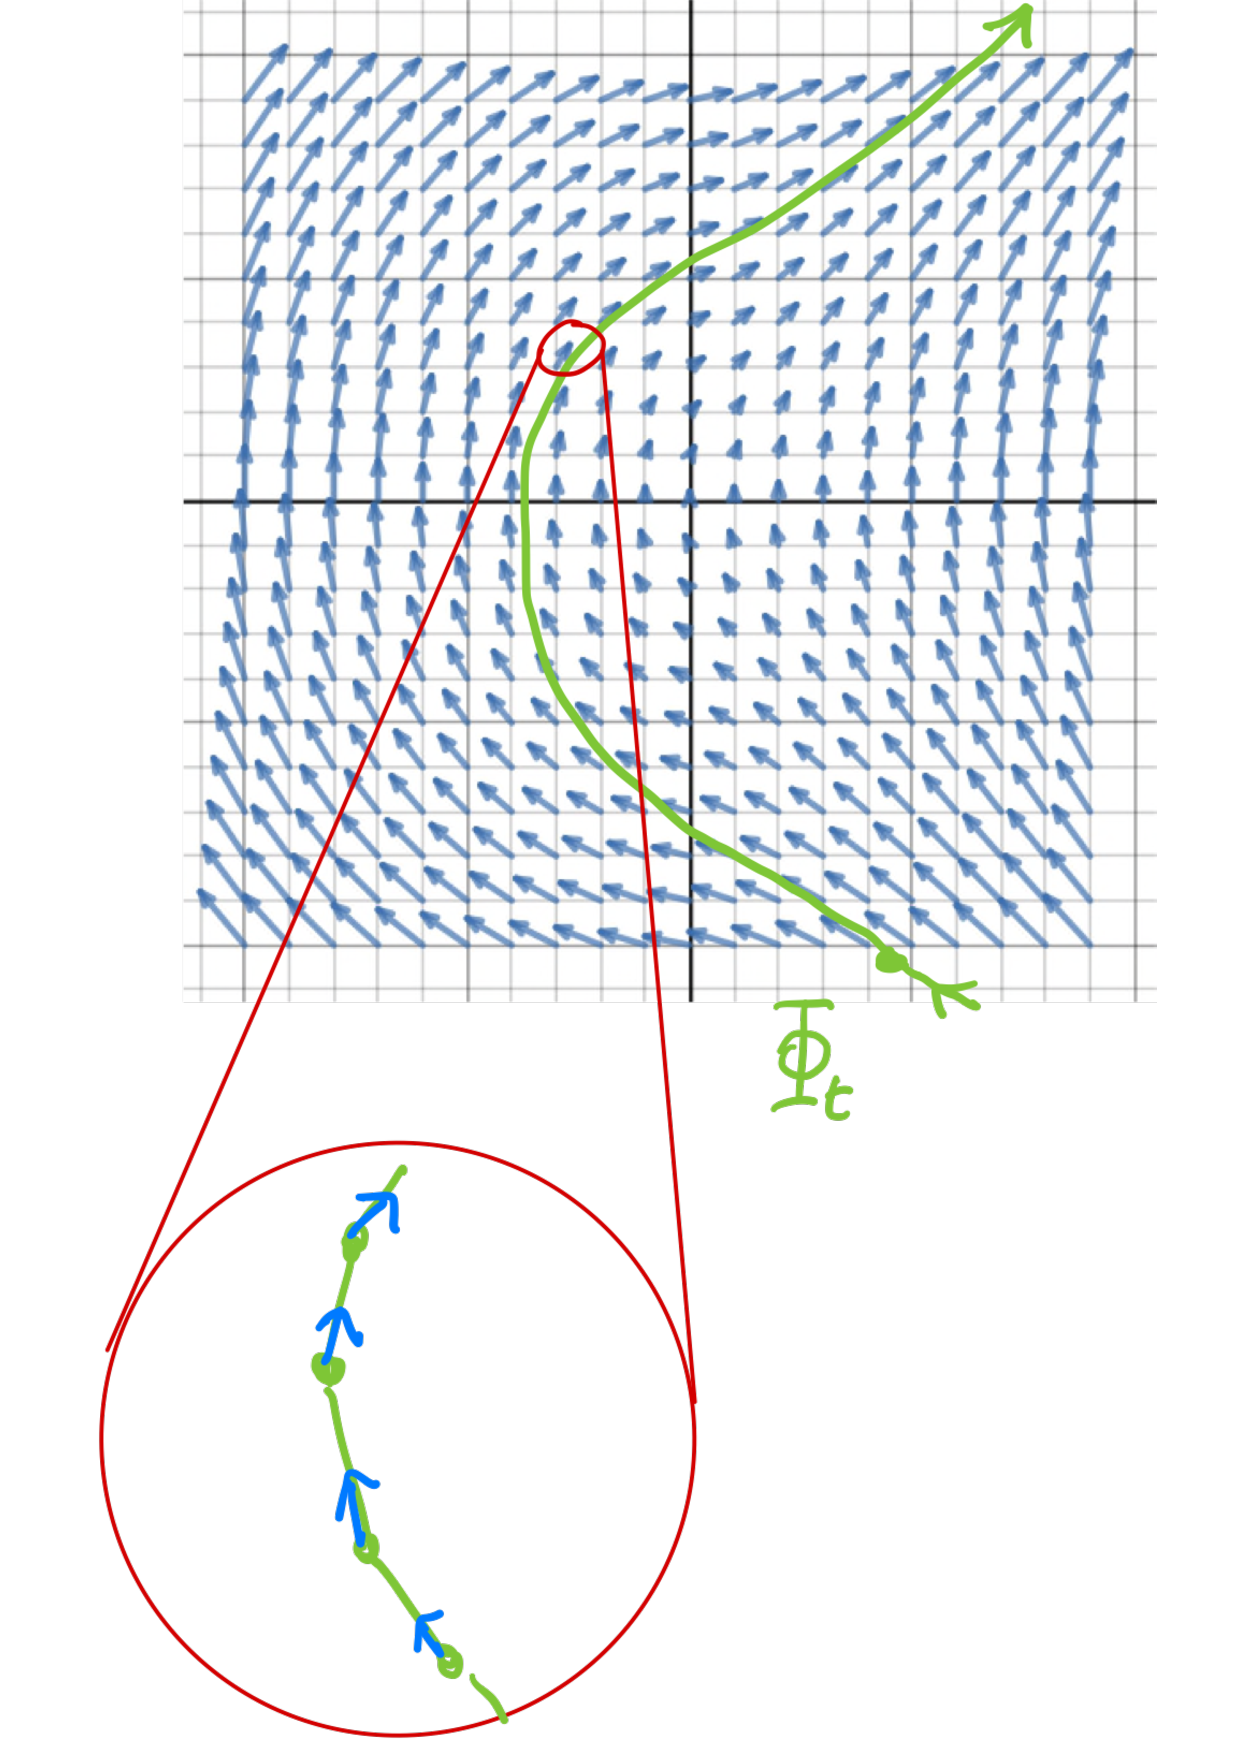
\includegraphics{3_1-vfield-infgen.pdf}
    \label{fig:3_1-vfield-infgen}
    \caption{One can think of a flow as a sequence of many infinitesimal straight motions determined by the value of the vector field, that is where ``infinitesimal generator'' comes from. We will soon make this rigorous.}
  \end{marginfigure}
  If $\{\Phi_t\}$ is a one-parameter group of diffeomorphisms, then we define its \emph{infinitesimal generator} as the (complete) vector field
  \marginnote{In a more compact form, we have just written $X_p = \frac{d}{dt}|_{t=0}\Phi_t(p)$.}
  \begin{equation}\label{eq:infgen}
    X_p := d\Phi_{(0,p)}\left(\frac{\partial}{\partial t}\Big|_{(0,p)}\right).
  \end{equation}
  Then the flow of $X$ is simply the one-parameter group $\Phi_t$.

  Always keep in mind that \eqref{eq:infgen} is just a ``scary'' way to write $X_p := \Phi_p'(0)$ where the role of the differential and the nature of the vector field are more explicit.
\end{definition}

The definition above, in fact, contains the proof of the following fact.
\begin{proposition}
  Let $M$ be a smooth manifold. There is a bijective correspondence between one-parameter groups of diffeomorphisms (i.e. global flows) and complete vector fields.
\end{proposition}

\begin{notation}
  Since by construction
  \begin{equation}
    \frac{d}{d t}\Phi_t(p) = X(\Phi_t(p)), \quad
    \Phi_0(p) = p, \quad \forall p\in M,
  \end{equation}
  it is often convenient to use the exponential notation
  \begin{equation}
    e^{t X} := \Phi^X_t, \quad t\in\R,
  \end{equation}
  to denote the flow of a vector field $X$.
\end{notation}

\begin{exercise}
  Show that the exponential defined above satisfies the following properties
  \begin{align}
    &e^{0X} = \id_M, \quad (e^{tX})^{-1} = e^{-tX}, \\
    &e^{t X}\circ e^{s X}= e^{(t+s)X},\\
    &\frac{d}{d t} e^{tX} (p) = X(e^{tX}(p)), \quad \forall p\in M.
  \end{align}

  Moreover, if $X(x) = Ax$ is a linear vector field on $\R^n$, that is $A$ is a $n\times n$-matrix, then the corresponding flow $\Phi_t$ is the matrix exponential $\Phi_t(x) = e^{Ax}$.
\end{exercise}

There are a few cases in which we can guarantee completeness, let's have a brief look.

\begin{lemma}\label{lemma:charactCompleteVF}
  Let $X\in\fX(M)$ and assume that there exists $\epsilon >0$ such that $(-\epsilon, \epsilon)\subset I_p$ for all $p \in M$.
  Then $X$ is complete.
\end{lemma}
\begin{proof}
  Assume that this is not the case, then there is some $p\in M$ such that either $t^+(p) < \infty$ or $t_-(p)>-\infty$.
  Say that $t^+(p) < \infty$ (the other case is nearly identical).
  
  Choose $t_0$ such that $t^+(p) - t_0 < \epsilon$ and set $p_0 = \gamma_p(t_0)$. By assumption, $\gamma_{p_0}(t)$ is defined for all $t\in(-\epsilon, \epsilon)$. Consider the curve
  \begin{equation}
    \gamma(t) := \begin{cases}
      \gamma_p(t), & t\in I_p,\\
      \gamma_{p_0}(t-t_0), & |t-t_0|<\epsilon.
    \end{cases}
  \end{equation}
  The two definitions coincide on the overlap as
  \begin{equation}
    \gamma_{p_0}(t-t_0) = \Phi_{t-t_0}(p_0) = \Phi_{t-t_0}\circ\Phi_{t_0}(p) = \Phi_t(p) = \gamma_p(t),
  \end{equation}
  but $\gamma$ is an integral curve for $X$ through $p$ which is defined on $(t^-(p), t_0+\epsilon)$.
  Since $t_0 + \epsilon > t^+(p)$, this contradict the maximality of $I_p$.
\end{proof}

\begin{corollary}
  Let $X\in\fX(M)$ be a vector field with compact support. The $X$ is complete.
\end{corollary}
\begin{proof}[Sketch of the proof.]
  Use the compactness to pick a finite covering of the support, define the local flow on the covering and then pick the smallest $\epsilon$ (out of the finitely many).
\end{proof}

\begin{corollary}
  If $M$ is compact\footnote{A compact manifold without boundary is called \emph{closed manifold}.}, then every vector field has compact support.
\end{corollary}

In the same fashion as Lemma~\ref{lemma:charactCompleteVF}, one can characterize non-complete vector fields.

\begin{lemma}\label{lemma:charactNotCompleteVF}
  Let $K\subset \circ M$ compact and $p\in K$.
  If $t^+(p) < \infty$, then there exists $0<\tau<t^+(p)$ such that $\gamma_p(t)\not\in K$ for all $t\in (\tau, t^+(p))$.
  An analogous statement holds if $t^-(p) > -\infty$.
\end{lemma}

\begin{exercise}
  Prove Lemma~\ref{lemma:charactNotCompleteVF}.
\end{exercise}

In other words, a maximal integral curve can not ``end'' inside a compact set that doesn't contain boundary points.
Thus, if a solution does not exist for all times, then it must either run to infinity in finite time\footnote{Recall Example~\ref{ex:non-complete}} or hit the boundary of $M$.

A natural question, at this point, is what happens when we map integral curves to different manifolds via diffeomorphisms, after all it looks like the mapping to euclidean spaces via the charts behaves quite nicely.

\begin{proposition}\label{prop:conjpfX}
  Let $F: M \to N$ be a diffeomorphism between smooth manifolds, $X\in\fX(M)$ a vector field and $\gamma:I\to M$ an integral curve of $X$. Then $F\circ\gamma : I \to N$ is an integral curve of $F_* X$.

  If $X$ is complete, we then have
  \begin{equation}
    F\circ\Phi_t^X = \Phi_t^{F_* X}\circ F.
  \end{equation}
  \marginnote[-6em]{Sometimes to understand what one is doing, it may be convenient to rewrite things in different forms, for example I find the following quite clarificatory \begin{equation}\label{eq:conjpfX}\Phi_t^{F_* X} = F \circ \Phi_t^X \circ F^{-1},\end{equation}}
\end{proposition}
\begin{proof}
  We only need to show that the two curves satisfy the same ODE.
  \begin{align*}
    d(F\circ \gamma)_t 
    &= dF_{\gamma(t)} \circ d\gamma_t \\
    &= dF_{\gamma(t)} \circ (X \circ \gamma)_t \\
    &= \LaTeXunderbrace{dF_{\gamma(t)} \circ X \circ F^{-1}} \circ F \circ \gamma(t) \\
    &= (F_* X) \circ (F\circ \gamma)(t) \\
    &= (F_* X)_{F\circ\gamma(t)}.
  \end{align*}
\end{proof}

\begin{remark}
  One particularly interesting consequence of Proposition~\ref{prop:conjpfX} in conjunction with the exponential notation is the following:
  \begin{equation}\label{eq:expdiff}
    \left(e_*^{tX} Y\right)_q =
    \frac{d}{ds}\Big|_{s=0} \exp\left(s\, e_*^{tX} Y\right)_q =
    \frac{d}{ds}\Big|_{s=0} e^{tX}\circ e^{sY}\circ e^{-t X}(q),
  \end{equation}
  where we are using the definition of integral flow in the first equality and \eqref{eq:conjpfX} in the second.
  This turns out to be rather useful for proofs and computations.  
\end{remark}

\begin{exercise}
  Use Theorem~\ref{thm:liealgiso} to show that the Lie bracket is the infinitesimal version of the pushforward of the second vector field along the flow of the first one, that is,
  \begin{equation}\label{def:liebracketsecondversion}
    [X,Y]\big|_q = \frac{\partial}{\partial t}\Big|_{t=0} (e_*^{-t X} Y)_q
  \end{equation}
 \textit{\small Hint: the identity $(F_* X)f = X(f\circ F)\circ F^{-1}$ and a Taylor expansion can help.}
\end{exercise}

\begin{remark}
  Equation~\eqref{def:liebracketsecondversion} and \eqref{eq:expdiff} imply that
  \begin{equation}\label{eq:lbddr}
    [X,Y]_q = \frac{\partial^2}{\partial s \partial t}\Big|_{t=s=0}e^{-tX}\circ e^{sY}\circ e^{t X}(q).
  \end{equation}
\end{remark}

With this we can show that the Lie bracket of two vector fields is zero (i.e., they commute as operator on functions) if and only if their flows commute, that is $\Phi^X_t \circ \Phi^Y_s = \Phi^Y_s\circ \Phi^X_t$ for all $t,s\in\R$.

\begin{proposition}
  Let $M$ be a smooth manifolds and $X,Y\in\fX(M)$. Then $[X,Y]=0$ if and only if their flows commute.
\end{proposition}
\begin{proof}
  First we show that $[X,Y] = 0$ implies that
  \begin{equation}\label{eq:intcurvconst}
    e^{-tX}_*Y = Y \quad \forall t\in\R.
  \end{equation}
  To this end, we are going to use \eqref{def:liebracketsecondversion} to show that $0 = [X,Y] = \frac{\partial}{\partial t}\Big|_{t=0} e_*^{-t X} Y$ implies that $\frac{\partial}{\partial t} e_*^{-t X} Y = 0$ for all $t\in\R$ (i.e., it is a constant map).
  Indeed, for any $t$,
  \begin{align}
    \frac{\partial}{\partial t} e_*^{-t X} Y
    &= \frac{\partial}{\partial \epsilon} \Big|_{\epsilon = 0} e_*^{-(t+\epsilon) X} Y
    = \frac{\partial}{\partial \epsilon} \Big|_{\epsilon = 0} e_*^{-t X}e_*^{-\epsilon X} Y\\
    &= e_*^{-tX} \frac{\partial}{\partial \epsilon} \Big|_{\epsilon = 0} e_*^{-\epsilon X} Y
    = e_*^{-tX} [X,Y] = 0.
  \end{align}
  
  $(\Longrightarrow)$ Fix $t\in\R$. We are going to show that $\Phi_s := e^{-tX}\circ e^{sY}\circ e^{tX}$ is the flow of $Y$, i.e. $\Phi_s = = e^{sY}$.
  We can use the previous trick, \eqref{eq:intcurvconst} and \eqref{eq:expdiff} to get, for any $s\in\R$,
  \begin{align}
    \frac{\partial}{\partial s} \Phi_s
    &= \frac{\partial}{\partial \epsilon} \Big|_{\epsilon = 0} e^{-tX}\circ e^{(s+\epsilon) Y}\circ e^{tX} \\
    &= \LaTeXunderbrace{\frac{\partial}{\partial \epsilon} \Big|_{\epsilon = 0} e^{-tX}\circ e^{\epsilon Y}\circ e^{tX}}_{e^{-tX}_* Y} \circ \LaTeXunderbrace{e^{-tX}\circ e^{s Y}\circ e^{tX}}_{\Phi_s} \\
    &= e^{-tX}_* Y \circ \Phi_s = Y \circ \Phi_s.
  \end{align}
  That is, $e^{-tX}\circ e^{sY}\circ e^{tX} = e^{sY}$ which is equivalent to the claim.

  $(\Longleftarrow)$ Let $f\in C^\infty(M)$, by \eqref{eq:lbddr} we have
  \begin{align}
    [X,Y]_q &= \frac{\partial^2}{\partial s \partial t}\Big|_{t=s=0}e^{-tX}\circ e^{sY}\circ e^{t X}(q)\\
    &= \frac{\partial^2}{\partial s \partial t}\Big|_{t=s=0} e^{sY} = 0.
  \end{align}
\end{proof}

\begin{exercise}
  Let $M$ be a smooth manifolds and $X,Y\in\fX(M)$.
  Define $(\ad X) Y := [X,Y]$.
  Use the semigroup property\footnote{We have shown it at the beginning of the previous proof!}
  \begin{equation}
    \frac{\partial}{\partial t} e_*^{tX} Y = e_*^{tX}[X,Y],
  \end{equation}
  to deduce the following \emph{formal} series expansion:
  \begin{align}
    e_*^{-tX} Y
    &= \sum_{n=0}^\infty \frac{t^n}{b!}(\ad X)^n Y \\
    &= Y + t[X,Y] + \frac{t^2}{2}[X, [X, Y]] + \frac{t^3}{6} [X,[X,[X,Y]]] + \cdots.
  \end{align}
\end{exercise}

After this parenthesis, let's go back to our final objective: we can finally justify our comment in Figure~\ref{fig:3_1-vfield-infgen}.
The following theorem shows that every flow $\Phi^X$ admits local coordinates on its support which map it into a linear flow.

\begin{definition}
  Let $M$ be a smooth manifold and $x\in\fX(M)$. 
  The \emph{support of $X$} is defined as
  \begin{equation}
    \supp(X):=\overline{\left\lbrace p\in M \;\mid\; X_p\neq 0 \in T_p M\right\rbrace}\subset M.
  \end{equation}
  Points $p\in\supp(X)$ are called \emph{regular points of $X$}.
  The points $p\in M\setminus\supp(X)$, i.e. such that $X_p = 0$, are the \emph{fixed points (or equilibrium points) of $X$}: for such points the unique integral curve through $p$ is $\gamma(t) \equiv p$ for all $t\in\R$. 
\end{definition}

\begin{theorem}[Normal form of a flow away from the fixed points]
  Let $M$ be a smooth manifold, $X\in\fX(M)$ and $p\in\supp(X)\subset M$.
  Then, there exists a chart $(U, \phi)$ with $p\in U$ such that
  \begin{equation}
    \phi_* X = L,
  \end{equation}
  where $L$ is the linear drift defined in Example~\ref{example:lineardrift}.
  Thus, locally,
  \begin{equation}
    \Phi_t^X = \phi^{-1} \circ \Phi_t^L \circ \phi.
  \end{equation}
\end{theorem}
\begin{proof}
  Choose a coordinate patch $(U_1, \psi)$ around $p$ (so $\psi(p) = 0$) such that $\psi_* X(0) = (1,0,0,\ldots, 0)$.
  By continuity of $\psi_*X\in \fX(\psi(U_1))$, we can always restrict to a smaller neighbourhood $V_2\subset \psi(U_1)$ on which $(\psi_*X)^1(q) > \frac12$ for all $q\in V_2$.

  Our objective is to interpolate $\psi_* X$ on $V\subset V_2$ and $L$ on $V_2^c$ to obtain a new vector field $\widetilde{L}$ on all of $\R^n$ which is diffeomorphic to $\widetilde{L}$.
  If $\Omega:\R^n\to\R^n$ is such diffeomorphism, i.e. $\Omega_* \tilde  L = L$, then $\phi = \Omega\circ\psi$ is the chart we are looking for: indeed, on $U=\psi^{-1}(V)$ we have $\phi_* X = \Omega_*\psi_*X = \Omega_* \widetilde{L} = L$.

  \newthought{Interpolated vector field $\widetilde{L}$}. Let $V\subset V_2$ be an open set around $0$. Pick a cutoff function $\chi\in C^\infty(\R^n)$ such that $\chi(x) = 1$ for $x\in U$ and $\chi(x) =0$ for $x\in U_2^c$.
  Then the interpolating vector field is immediately obtained as
  \begin{equation}
    \widetilde{L} = \chi \psi_*X + (1-\chi)L \in \fX(\R^n).
  \end{equation}
  \begin{marginfigure}
    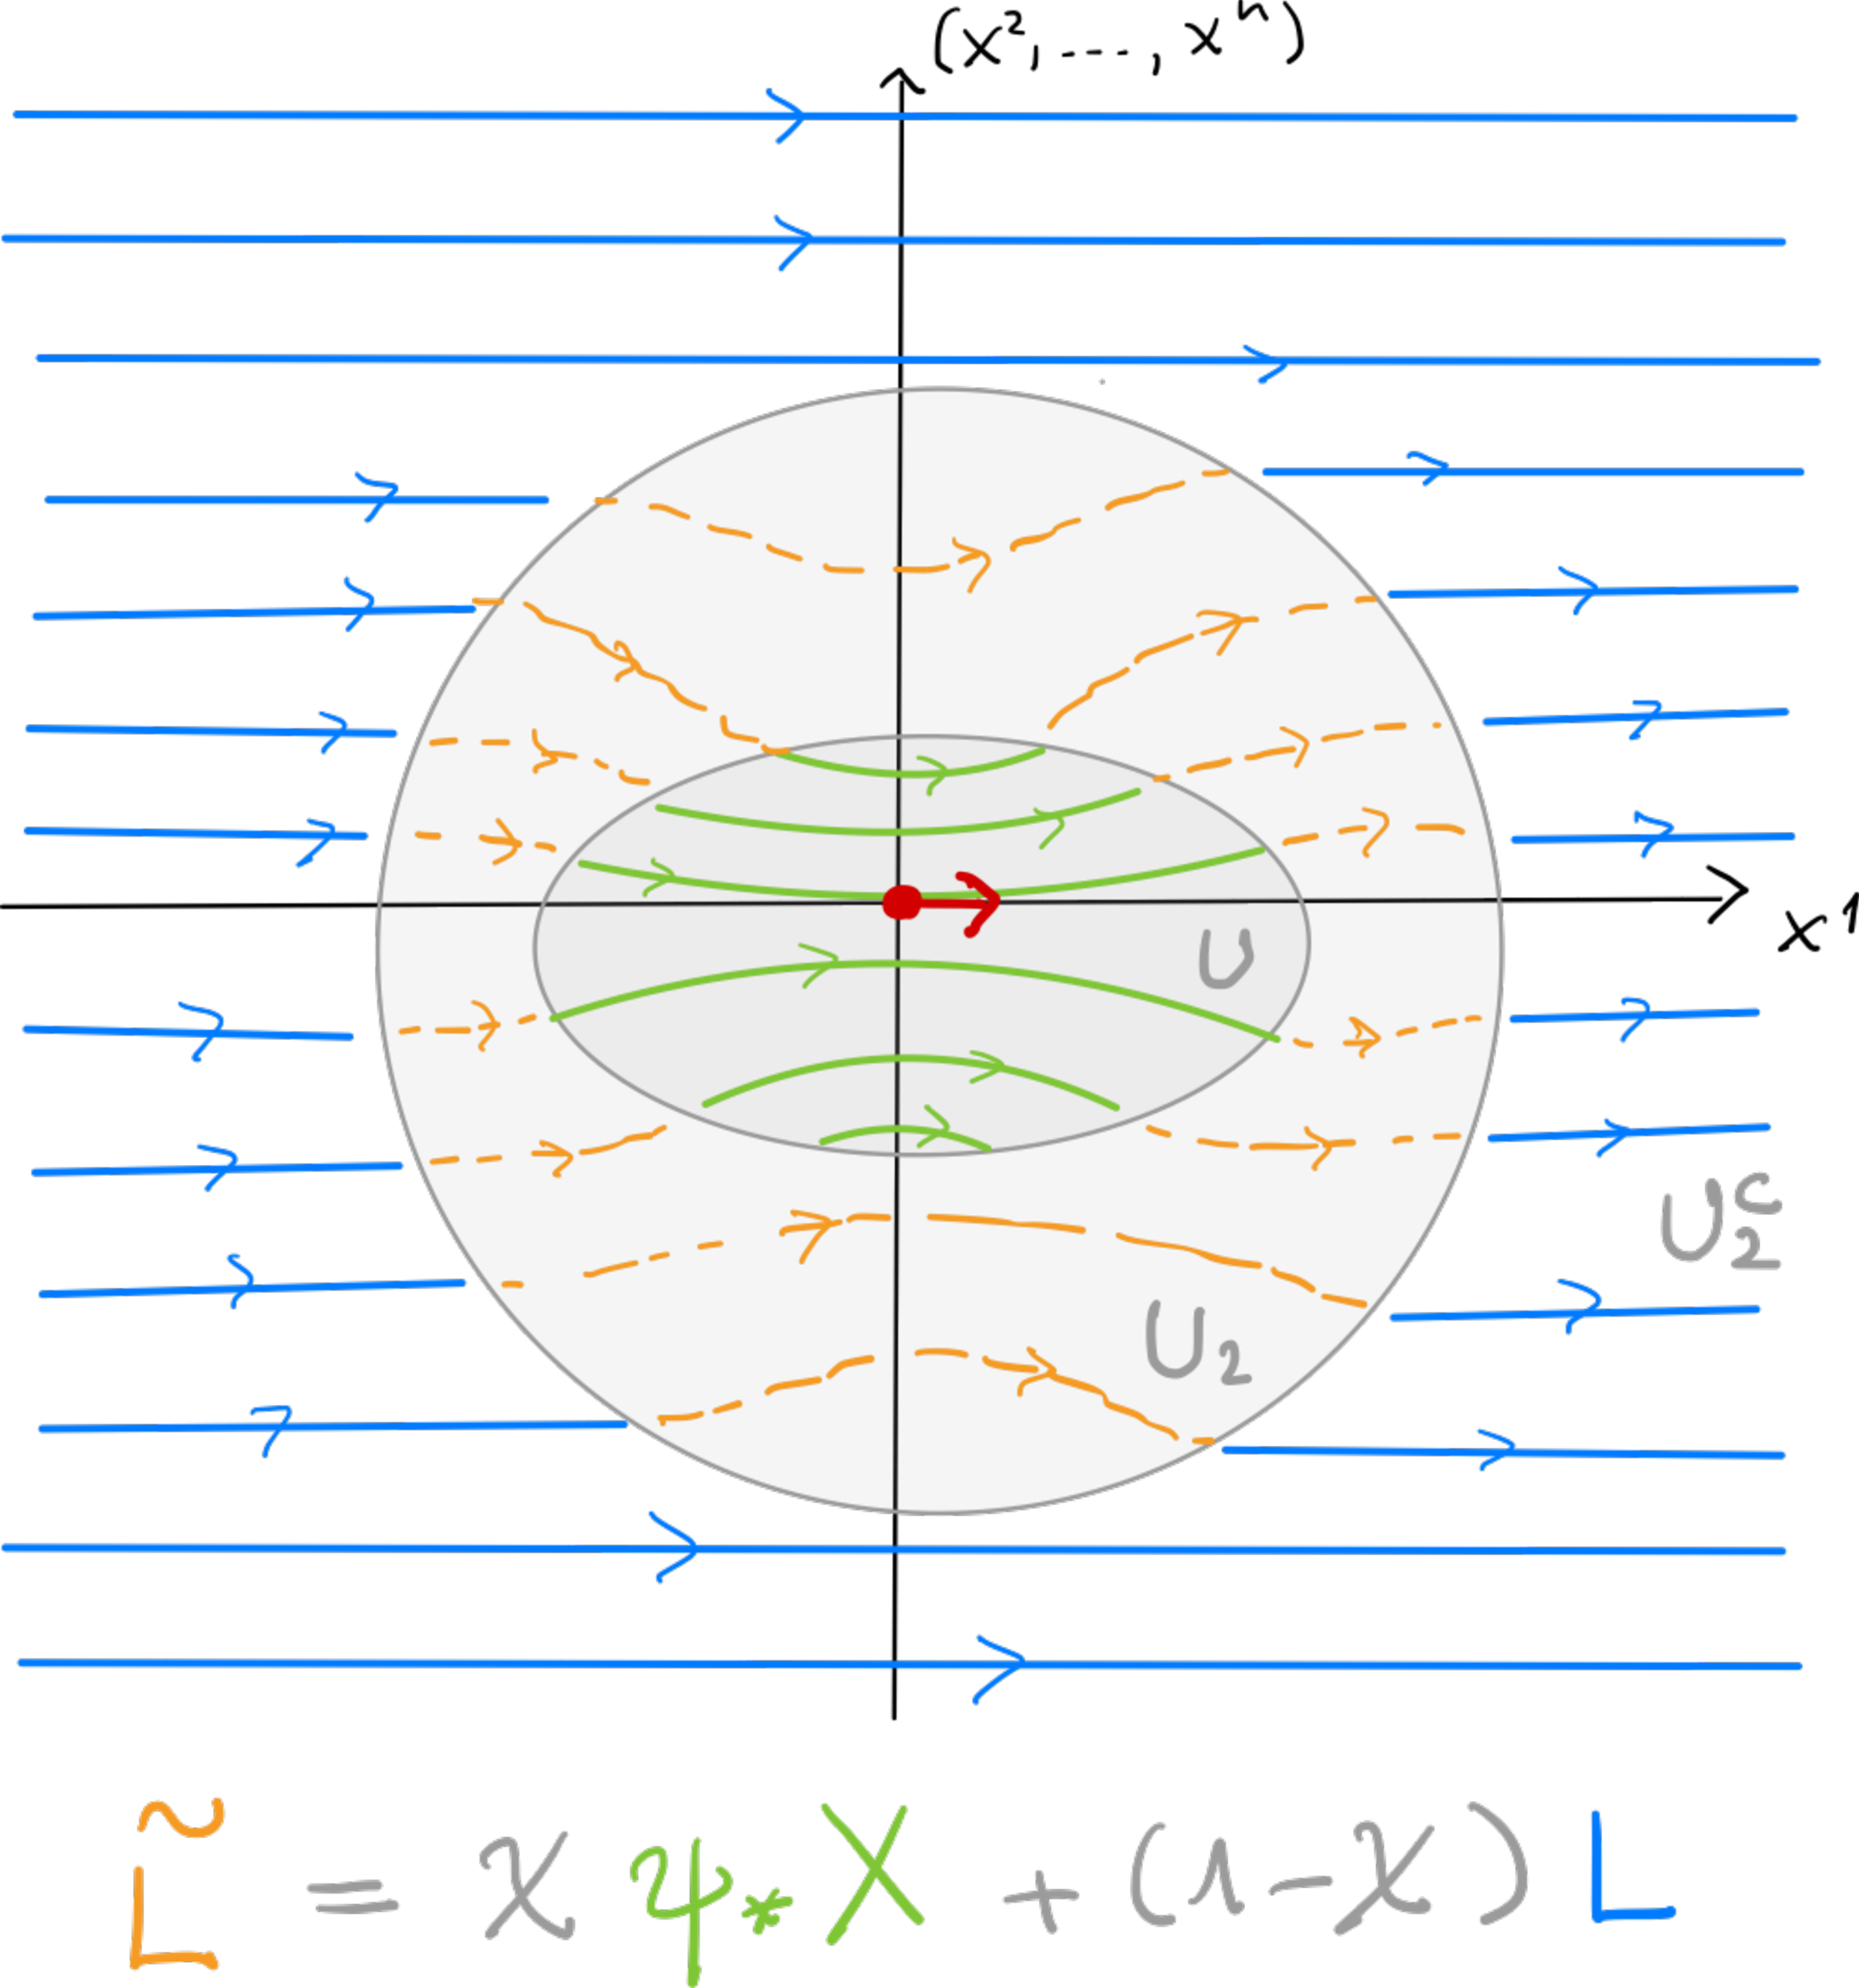
\includegraphics{3_2-vfield-patched.pdf}
  \end{marginfigure}
  Clearly its flow $\Phi_t^{\widetilde{L}}$ is global as $\R^n$ has no boundary and the regularity of the functions involved implies that no integral curve can escape to infinity in finite time.

  \newthought{Diffeomorphism $\Omega$}. We will now show that
  \begin{equation}
    \Omega = \lim_{t\to\infty} \Phi_{-t}^L \circ \Phi_t^{\widetilde{L}}
  \end{equation}
  exists and defines a diffeomorphism such that $\Omega_* \widetilde{L} = L$.
  \marginnote{It is interesting to compare $\Omega$ with the so called M\o{}ller transformations in scattering theory (cf. \cite[Chapter 12.2]{book:knauf}).}
  Since by construction $(\Phi_t^{\widetilde{L}}(q))^1 \geq q^1 + \frac12$, every integral curve leaves $V_2$ after a finite time.
  So, on compact sets $K\subset\R^n$, there is a finite time $t_0(K)$ after which the limit is attained (can you explain why?):
  \begin{equation}
    \lim_{t\to\infty} \Phi_{-t}^L \circ \Phi_t^{\widetilde{L}}\Big|_K = \Phi_{-t_0}^L \circ \Phi_{t_0}^{\widetilde{L}}.
  \end{equation}
  Thus, $\Omega$ is a well defined diffeomorphism.
  Moreover,
  \begin{align}
    \Omega \circ \Phi^{\widetilde{L}}_t &= \lim_{s\to\infty} \Phi_{-s}^L \circ \Phi^{\widetilde{L}}_s \circ \Phi^{\widetilde{L}}_t \\
    &= \lim_{s\to\infty} \Phi_{-s}^L \circ \Phi^{\widetilde{L}}_{s+t} \\
    &= \lim_{\tau\to\infty} \Phi_{t-\tau}^L \circ \Phi^{\widetilde{L}}_s \circ \Phi^{\widetilde{L}}_\tau \\
    &= \lim_{\tau\to\infty} \Phi_{t}^L \circ \Phi_{-\tau}^L \circ \Phi^{\widetilde{L}}_s \circ \Phi^{\widetilde{L}}_\tau = \Phi_t^L \circ \Omega,
  \end{align}
  and therefore the flows are diffeomorphic.
  In particular, we also have $\Phi_p^{\widetilde{L}} = \Omega^{-1} \circ \Phi^L_{\Omega(x)}$.
  Differentiating this last equation we get
  \begin{align}
    (\widetilde{L} \circ \Phi^{\widetilde{L}})_p &= d\Phi^{\widetilde{L}}_p \\
    &= d\Omega^{-1}_{\Phi^L_{\Omega(x)}} \circ d\Phi^L_{\Omega(x)} \\
    &= d\Omega^{-1}_{\Phi^L_{\Omega(x)}} \circ (L \circ \Phi^L)_{\Omega(x)},
  \end{align}
    which, at $t=0$, gives $\widetilde{L} = d\Omega^{-1} \circ L \circ \Omega = \Omega^{-1}_* L$.
\end{proof}

\begin{remark}[Linearisation of a vector field at a fixed point]
  Away from the fixed points, the previous theorem, tells us that the flow is locally linear.
  Near a fixed point we can describe the flow in terms of the \emph{linearisation} of the associated vector field.

  If $X\in\fX(M)$ and $p_0\in M$ with $X_{p_0} = 0$. On a chart $\phi$ centred at $p_0$ with local coordinates $(x^i)$, let $\tilde X = \phi_* X$.
  Then we have
  \begin{equation}
    \tilde X_x = \underbrace{\tilde X_0}_{=0} + d\tilde X_0 x + \cO(\|x\|^2) = d\tilde X_0 x + \cO(\|x\|^2).
  \end{equation}
  Close to $x=0$ we can thus approximate $\tilde X_x$ by its linearisation $ d\tilde X_0 x$.
  %
  Qualitatively, the behaviour close to the fixed point is determined by the eigenvalues\footnote{Note that thanks to the compatibility conditions, the linearisations of $X$ at different charts are similar matrices, and thus the spectrum of $d\tilde X_0 x$ is independent of the choice of local coordinates.} of $d\tilde X_0 x$ and their geometric multiplicities (cf. \cite[Figure 9.8]{book:lee}). This is the same as you have seen in the euclidean case \cite[Chapter 5.3]{book:knauf}.
\end{remark}

\begin{tcolorbox}
For simplicity in the rest of the course we will discuss only global flows.
But keep in mind that all results hold also for local flows as long as one restricts the domains appropriately.
\end{tcolorbox}
